\documentclass{article}
\usepackage{amsmath}
\usepackage{amssymb}
\usepackage{graphicx}
\usepackage{tikz}
\usepackage{pgfplots}
\usepackage{float}
\usepackage{subcaption}
\usepackage{geometry}

\geometry{a4paper, margin=1in}

% Define example environment
\newenvironment{example}[1]{
    \begin{trivlist}
    \item[\textbf{Example:}] #1
    \vspace{0.5em}
}{
    \end{trivlist}
    \vspace{1em}
}

\pgfplotsset{compat=1.18}
\usetikzlibrary{patterns,decorations.pathreplacing}

\title{Lecture 8 Examples}
\author{Signals and Systems Course}
\date{}

\begin{document}

\maketitle

\begin{example}[1. Fourier Series Coefficients using Linearity Property]
\textbf{Problem:}
Find Fourier Series representation for periodic signal $z(t)$ with period $T=1$.

\begin{figure}[H]
\centering

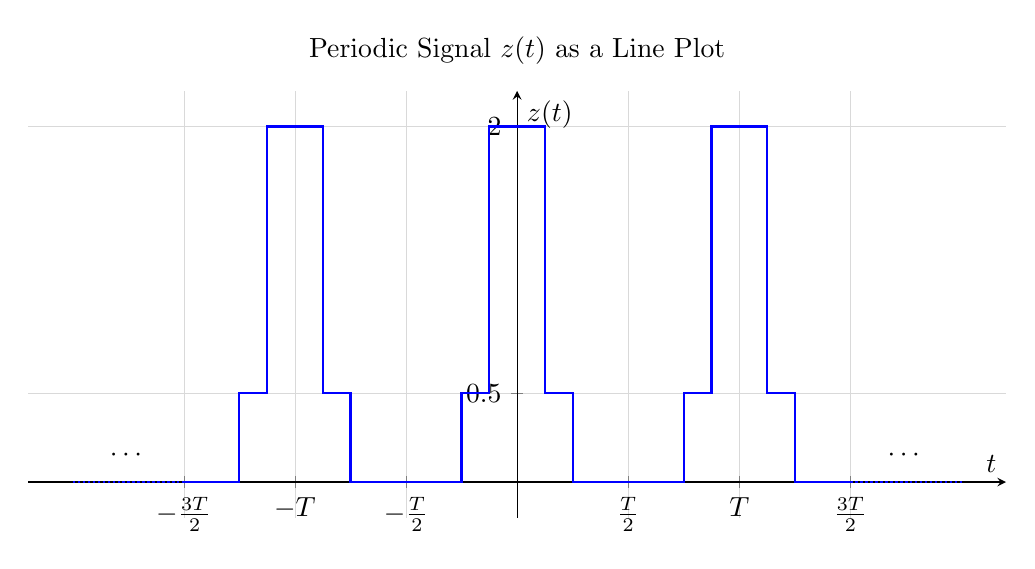
\begin{tikzpicture}
	\begin{axis}[
		% Set the overall style
		width=14cm,
		height=7cm,
		title={Periodic Signal $z(t)$ as a Line Plot},
		xlabel={$t$},
		ylabel={$z(t)$},
		% Position axes at the origin
		axis lines=middle,
		% Set axis limits
		xmin=-2.2, xmax=2.2,
		ymin=-0.2, ymax=2.2, % Lowered ymin slightly for better axis visibility
		% Set symbolic ticks for the period T=1
		xtick={-1.5, -1, -0.5, 0.5, 1, 1.5},
		xticklabels={$-\frac{3T}{2}$, $-T$, $-\frac{T}{2}$, $\frac{T}{2}$, $T$, $\frac{3T}{2}$},
		ytick={0.5, 2},
		% Add a grid
		grid=major,
		grid style={line width=.1pt, draw=gray!30},
		no marks,
		]
		
		% --- Plot each cycle as a single, continuous outline ---
		
		% Cycle 1 (Centered at t = -1)
		\addplot[blue, thick] coordinates {
			(-1.5,0) (-1.25,0) (-1.25,0.5) (-1.125,0.5) (-1.125,2) 
			(-0.875,2) (-0.875,0.5) (-0.75,0.5) (-0.75,0) (-0.5,0)
		};
		
		% Cycle 2 (Centered at t = 0)
		\addplot[blue, thick] coordinates {
			(-0.5,0) (-0.25,0) (-0.25,0.5) (-0.125,0.5) (-0.125,2) 
			(0.125,2) (0.125,0.5) (0.25,0.5) (0.25,0) (0.5,0)
		};
		
		% Cycle 3 (Centered at t = 1)
		\addplot[blue, thick] coordinates {
			(0.5,0) (0.75,0) (0.75,0.5) (0.875,0.5) (0.875,2) 
			(1.125,2) (1.125,0.5) (1.25,0.5) (1.25,0) (1.5,0)
		};
		
		% --- Indicate that the pattern continues ---
		\draw[blue, thick, densely dotted] (axis cs:1.5, 0) -- (axis cs:2, 0);
		\node at (axis cs:1.75, 0.15) {$\cdots$};
		\draw[blue, thick, densely dotted] (axis cs:-2, 0) -- (axis cs:-1.5, 0);
		\node at (axis cs:-1.75, 0.15) {$\cdots$};
		
		% Add period label for one period
		\draw[<->, thick] (axis cs:-0.5, -0.3) -- (axis cs:0.5, -0.3) node[midway, below=2pt] {Period $T = 1$};
		
	\end{axis}
\end{tikzpicture}
\caption{The periodic signal $z(t)$.}
\label{fig:z_t}
\end{figure}

\textbf{Solution:}
Decompose: $z(t) = \frac{3}{2}x(t) + \frac{1}{2}y(t)$

\begin{figure}[H]
\centering
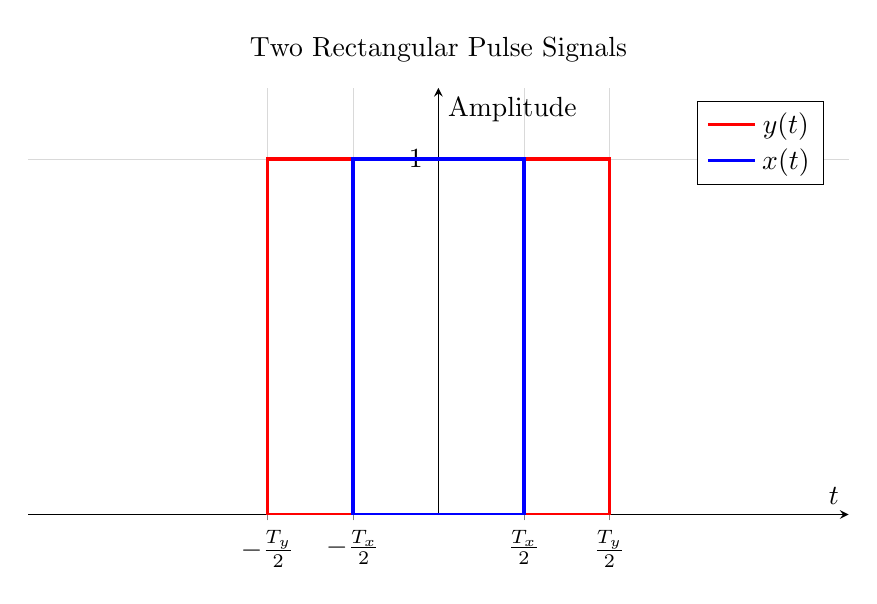
\begin{tikzpicture}
	\begin{axis}[
		% Set the overall style
		width=12cm,
		height=7cm,
		title={Two Rectangular Pulse Signals},
		xlabel={$t$},
		ylabel={Amplitude},
		% Position axes at the origin
		axis lines=middle,
		% Set axis limits to focus on the signals
		xmin=-0.6, xmax=0.6,
		ymin=0, ymax=1.2,
		% Set symbolic ticks for the pulse widths and amplitude
		xtick={-0.25, -0.125, 0.125, 0.25},
		xticklabels={$-\frac{T_y}{2}$, $-\frac{T_x}{2}$, $\frac{T_x}{2}$, $\frac{T_y}{2}$},
		ytick={1},
		yticklabels={$1$},
		% Add a grid
		grid=major,
		grid style={line width=.1pt, draw=gray!30},
		% Position the legend
		legend pos=north east,
		]
		
		% Use \addlegendimage to create legend entries for \draw commands
		\addlegendimage{red, very thick}
		\addlegendentry{$y(t)$}
		\addlegendimage{blue, very thick}
		\addlegendentry{$x(t)$}
		
		% Draw the wider pulse (y(t)) first so it's in the background
		\draw[red, very thick]
		(axis cs:-0.25, 0) -- (axis cs:-0.25, 1) -- (axis cs:0.25, 1)
		-- (axis cs:0.25, 0) -- cycle;
		
		% Draw the narrower pulse (x(t))
		\draw[blue, very thick]
		(axis cs:-0.125, 0) -- (axis cs:-0.125, 1) -- (axis cs:0.125, 1)
		-- (axis cs:0.125, 0) -- cycle;
		
	\end{axis}
\end{tikzpicture}
\caption{The complex signal $z(t)$ is decomposed into two simpler periodic square waves.}
\label{fig:components}
\end{figure}

For $x(t)$ (pulse width $1/4$): $a_k = \frac{\sin(k\pi/4)}{k\pi}$ ($k \neq 0$), $a_0 = \frac{1}{4}$
For $y(t)$ (pulse width $1/2$): $b_k = \frac{\sin(k\pi/2)}{k\pi}$ ($k \neq 0$), $b_0 = \frac{1}{2}$

Combined: $c_k = \frac{3}{2}a_k + \frac{1}{2}b_k$

\textbf{Answer:} $c_k = \begin{cases} \frac{3}{2k\pi}\sin(k\pi/4) + \frac{1}{2k\pi}\sin(k\pi/2) & k \neq 0 \\ \frac{5}{8} & k=0 \end{cases}$
\end{example}

\end{document}